% Guion de estudio de la presentación final.
% Compilar desde esta carpeta con: latexmk -pdf guion.tex
% Las miniaturas salen de ../presentacion.pdf (exportado desde ../index.html).
\documentclass[11pt,a4paper]{article}

\usepackage[utf8]{inputenc}
\usepackage[T1]{fontenc}
\usepackage[spanish,es-noquoting,es-nodecimaldot]{babel}
\usepackage{tgpagella}
\usepackage{tgheros}
\usepackage{textcomp}
\usepackage{microtype}
\usepackage[a4paper,top=24mm,bottom=24mm,left=24mm,right=24mm]{geometry}
\usepackage{graphicx}
\usepackage{xcolor}
\usepackage{booktabs}
\usepackage{tabularx}
\usepackage{array}
\usepackage[shortlabels]{enumitem}
\usepackage{titlesec}
\usepackage{fancyhdr}
\usepackage[most]{tcolorbox}
\usepackage{hyperref}

% Colores de la presentación
\definecolor{tinta}{HTML}{13212E}
\definecolor{tinta2}{HTML}{3C4B59}
\definecolor{tenue}{HTML}{75828F}
\definecolor{linea}{HTML}{D3DBE1}
\definecolor{banda}{HTML}{E3EBF1}
\definecolor{ambar}{HTML}{C2661B}
\definecolor{ambarsuave}{HTML}{F6E7D8}
\definecolor{azul}{HTML}{1C5A8A}

\hypersetup{colorlinks=true, linkcolor=tinta, urlcolor=azul, pdftitle={Guion de la presentación final}}
\color{tinta}

\setlength{\parindent}{0pt}
\setlength{\parskip}{6pt}
\linespread{1.08}
\setlist{itemsep=3pt, topsep=4pt, leftmargin=16pt}

\newcommand{\pmd}{PM\textsubscript{2.5}}
\newcommand{\ug}{\textmu g/m\textsuperscript{3}}
\newcommand{\flecha}{\ensuremath{\rightarrow}}

% Títulos en letra sin serifa
\titleformat{\section}{\sffamily\Large\bfseries\color{tinta}}{\thesection}{10pt}{}
\titlespacing*{\section}{0pt}{18pt}{8pt}
\titleformat{\subsection}{\sffamily\large\bfseries\color{tinta}}{}{0pt}{}
\titlespacing*{\subsection}{0pt}{12pt}{4pt}

\pagestyle{fancy}
\fancyhf{}
\renewcommand{\headrulewidth}{0pt}
\fancyfoot[L]{\sffamily\footnotesize\color{tenue}Guion · Pronóstico de \pmd{} a un día}
\fancyfoot[R]{\sffamily\footnotesize\color{tenue}\thepage}

% Cajas
\newtcolorbox{idea}{enhanced, breakable, colback=banda, colframe=banda, arc=0pt, boxrule=0pt,
  left=10pt, right=10pt, top=8pt, bottom=8pt, borderline west={3pt}{0pt}{azul},
  fontupper=\small, before upper={\textsf{\textbf{\color{azul}Idea clave}}\par\smallskip}}
\newtcolorbox{preguntas}{enhanced, breakable, colback=ambarsuave, colframe=ambarsuave, arc=0pt, boxrule=0pt,
  left=10pt, right=10pt, top=8pt, bottom=8pt, borderline west={3pt}{0pt}{ambar},
  fontupper=\small, before upper={\textsf{\textbf{\color{ambar}Si preguntan}}\par\smallskip}}
\newcommand{\pr}[2]{\textbf{¿#1?}\par #2\par\medskip}

% Encabezado de cada diapositiva: número, título, tiempo y miniatura
% Quién presenta: se cambia con \presenta{...} antes de la primera diapositiva de cada parte
\newcommand{\quien}{}
\newcommand{\presenta}[1]{\renewcommand{\quien}{#1}}
\newcommand{\diapo}[3]{%
  \clearpage
  {\sffamily\small\color{tenue}Diapositiva #1 \quad·\quad #3 \quad·\quad \textcolor{ambar}{\textbf{Presenta: \quien}}}\par\vspace{2pt}
  {\sffamily\LARGE\bfseries #2\par}\vspace{10pt}
  \fcolorbox{linea}{white}{\includegraphics[page=#1,width=0.72\textwidth]{../presentacion.pdf}}\par\vspace{8pt}
}
\newcommand{\decir}{\subsection*{Qué decir}}

\begin{document}

% ================= PORTADA =================
\begin{titlepage}
  \vspace*{40mm}
  {\sffamily\small\color{tenue}Aprendizaje de Máquina Aplicado · Universidad EAFIT}\par\vspace{10pt}
  {\sffamily\fontsize{30}{36}\selectfont\bfseries Guion de la presentación\par}\vspace{8pt}
  {\Large Pronóstico de \pmd{} a un día por estación en el Valle de Aburrá\par}\vspace{24pt}
  {\color{tinta2}Lina Sofía Ballesteros Merchán\\Alejandro Ríos Muñoz\par}\vspace{6pt}
  {\color{tenue}Octubre de 2026\par}
  \vfill
  \begin{tcolorbox}[colback=banda, colframe=banda, arc=0pt, boxrule=0pt, left=12pt, right=12pt, top=10pt, bottom=10pt]
    \textsf{\textbf{Cómo usar este guion}}\par\smallskip
    Las diapositivas solo muestran la evidencia; lo que se explica está aquí. Empiecen por
    la historia en un minuto, las cifras clave y las palabras clave (primeras páginas): si
    las dominan, el resto se sigue solo. Después, cada diapositiva tiene su miniatura, el tiempo sugerido, qué
    decir con palabras sencillas, la idea que el público debe llevarse y cómo responder
    si preguntan. La exposición dura 15 minutos y quedan 5 para preguntas.
  \end{tcolorbox}
  \vspace{8pt}
  \begin{tcolorbox}[colback=ambarsuave, colframe=ambarsuave, arc=0pt, boxrule=0pt, left=12pt, right=12pt, top=10pt, bottom=10pt]
    \textsf{\textbf{Quién presenta qué}}\par\smallskip
    \renewcommand{\arraystretch}{1.2}
    \begin{tabularx}{\linewidth}{>{\bfseries}l X r}
    Lina & Diapositivas 1 a 8: introducción, datos y qué información usa el modelo & 7 min 15 s \\
    Alejandro & Diapositivas 9 a 15: modelos, evaluación, resultados y conclusiones & 7 min 45 s \\
    Los dos & Diapositiva 16: preguntas & 5 min \\
    \end{tabularx}
  \end{tcolorbox}
\end{titlepage}

% ================= HISTORIA =================
\section{La historia en un minuto}

En el Valle de Aburrá el aire se contamina con \pmd, unas partículas tan pequeñas que llegan
hasta el fondo de los pulmones. Como el valle es estrecho y rodeado de montañas, hay días en
que el aire queda atrapado y la contaminación sube. La norma colombiana fija un \emph{Nivel de
Prevención} a partir de 38~\ug{} y permite declararlo con anticipación si un pronóstico lo
indica.

Nos preguntamos si, con los datos públicos de SIATA, se puede pronosticar la contaminación de
mañana en cada estación. Para saber si el pronóstico sirve, lo comparamos con la regla más
simple posible: suponer que mañana será igual a hoy (la \emph{persistencia}). Esa regla es
difícil de superar, porque la contaminación cambia poco de un día al siguiente.

Entrenamos un modelo de aprendizaje automático con ocho años de datos de 16 estaciones y lo
pusimos a prueba en 2022--2025, años que no vio al aprender. El resultado: se equivoca un 18~\%
menos que la persistencia y logra avisar a tiempo 30 de los 123 días en que empezó un episodio,
algo que la persistencia nunca consigue. Añadir el clima ayuda, pero poco. Lo que más pesa en
el pronóstico es la contaminación del día anterior, igual que encontró un estudio previo del
valle. Al repetir la prueba de ese estudio, descubrimos que la regla simple casi lo igualaba, y
que nuestro modelo falla cuando llega un episodio más fuerte que todos los que conoció.

% ================= CIFRAS =================
\section{Las cifras que hay que saberse}

\renewcommand{\arraystretch}{1.25}
\begin{tabularx}{\textwidth}{>{\sffamily\bfseries}l X}
\toprule
\normalfont\textsf{Cifra} & \textsf{Qué significa} \\
\midrule
38~\ug & Donde empieza el Nivel de Prevención para el promedio de un día. \\
16 estaciones & Las que tienen datos casi completos de 2018 a 2025 (de 33 que ha tenido la red). \\
44.399 & Registros con los que se trabajó: una estación en un día, con el promedio de ese día y del siguiente. \\
0,805 & Qué tanto se parece la contaminación de mañana a la de hoy (1 sería idéntica). Por eso la persistencia es difícil de superar. \\
3,37 \flecha{} 2,74 & Error promedio de la persistencia y del modelo con clima, en \ug, en los años de prueba. \\
18~\% & Cuánto menos se equivoca el modelo que la persistencia (sin usar el clima). \\
0,027~\ug & Lo que mejora el error al añadir el clima: poco, pero real y en 14 de 16 estaciones. \\
30 de 123 & Inicios de episodio que el modelo avisa el día antes. La persistencia: ninguno. \\
$-$5,5~\ug & En los días de prevención, el modelo se queda corto en promedio por esta cantidad. \\
49,5~\% & Peso de la contaminación del día anterior en el pronóstico. El estudio previo encontró 34,2~\%. \\
8,6~\% & Peso de todo el clima junto en el pronóstico. \\
\bottomrule
\end{tabularx}

% ================= GLOSARIO =================
\section{Palabras clave, sin tecnicismos}

Si hay que usar un término técnico, digan primero la idea sencilla y después el nombre.

{\small
\begin{description}[style=nextline, leftmargin=0pt, labelsep=0pt, itemsep=2pt, font=\sffamily\bfseries]
\item[\pmd] Partículas de menos de 2,5 micras en el aire. Se mide su concentración en
  microgramos por metro cúbico (\ug).
\item[SIATA] El sistema público que mide la calidad del aire y el clima en el Valle de
  Aburrá, hora a hora, en estaciones repartidas por la región.
\item[Persistencia] La regla de suponer que mañana será igual a hoy. Es nuestra vara de
  medir: un modelo solo vale la pena si le gana.
\item[Inicio de episodio] El primer día en que una estación pasa los 38~\ug{} después de
  estar por debajo. Es el día en que un aviso sirve de verdad.
\item[Modelo (Gradient Boosting)] Un método que aprende de ejemplos pasados combinando
  muchos árboles de decisión: preguntas sencillas del tipo ``¿hoy estuvo por encima de 30?''.
  Cada árbol nuevo se dedica a corregir los errores de los anteriores.
\item[Aprendizaje supervisado de regresión] Aprender a predecir un número (la contaminación
  de mañana) a partir de ejemplos en los que ya sabemos la respuesta.
\item[Días anteriores (rezagos y ventanas)] Los valores de ayer, antier y así hasta hace
  seis días, y sus promedios de 3 y 7 días. Le dicen al modelo hacia dónde va la tendencia.
\item[Error promedio (MAE)] En promedio, por cuántos \ug{} se equivoca el pronóstico. Menos
  es mejor.
\item[Ajuste (R²)] Qué tanto sigue el pronóstico las subidas y bajadas reales, de 0 a 1.
  Depende mucho del periodo, así que no sirve para comparar estudios distintos.
\item[Intervalo de confianza] El rango en el que probablemente está la mejora real. Si no
  incluye el cero, la mejora no es casualidad. Lo calculamos remuestreando bloques de dos
  semanas, porque días seguidos se parecen entre sí.
\item[Examen final (origen móvil)] Cada año se predice con un modelo que solo aprendió de
  los años anteriores, como se usaría en la vida real. Los años 2019--2021 sirvieron para
  ajustar el modelo; 2022--2025 fueron el examen, y no se miraron para tomar decisiones.
\item[Mismo número de avisos] Para comparar con justicia, cada método avisa tantas veces
  como eventos hubo en los años anteriores. Así nadie gana solo por avisar más.
\item[SHAP] Una forma de repartir cada pronóstico entre los datos que lo produjeron, para
  saber cuánto pesó cada uno.
\item[Sin imputar] No rellenamos datos que faltan con valores inventados; el modelo sabe
  trabajar con huecos.
\end{description}
}

% ================= DIAPOSITIVAS =================
\presenta{Lina}
\diapo{1}{Portada}{30 segundos}
\decir
Lina nos presenta a los dos y dice el objetivo en una frase: pronosticar la contaminación por \pmd{}
de mañana en cada estación del Valle de Aburrá, usando los datos públicos de SIATA.

La curva de la derecha es real: es la contaminación promedio según la hora del día. Sube con
el tráfico de la mañana, hasta 25,8~\ug{} a las 8:00, y baja en la tarde, hasta 13,5 a las
3:00 p.\,m., cuando el aire se mezcla mejor.

\begin{idea}
La contaminación tiene un ritmo diario muy marcado, y eso ya sugiere que se puede anticipar.
\end{idea}

\diapo{2}{Un valle que atrapa el aire}{1 minuto}
\decir
El \pmd{} son partículas tan pequeñas, menos de 2,5 micras, que pasan las defensas de la nariz
y la garganta y llegan al fondo de los pulmones. En el valle se han relacionado con más
consultas por infecciones respiratorias, EPOC y asma.

El dibujo explica por qué el problema es peor aquí. El valle es estrecho y está rodeado de
montañas. Algunos días se forma una \emph{inversión térmica}: una capa de aire más caliente
arriba actúa como una tapa, el aire frío queda abajo y la contaminación no se puede escapar.

La barra de la derecha es la norma, la Resolución 2254 de 2017. El Nivel de Prevención empieza
en 38~\ug{} para el promedio de un día. La norma dice dos cosas que justifican el trabajo: los
niveles se evalúan en cada estación, y se pueden declarar con anticipación si un pronóstico lo
indica.

\begin{idea}
Anticipar importa por tres razones que se suman: la salud, la geografía del valle y una norma
que permite avisar con un pronóstico.
\end{idea}

\begin{preguntas}
\pr{El dibujo está a escala}{No, es un esquema para explicar la inversión térmica. La escala de
la norma tampoco está a proporción en el último tramo: la Emergencia empieza en 151~\ug.}
\pr{Esto reemplaza el monitoreo}{No. Le da al monitoreo una señal anticipada por estación.}
\end{preguntas}

\diapo{3}{El problema y las dos preguntas}{1 minuto}
\decir
El monitoreo dice qué contaminación hubo; para prevenir hay que saber cuál viene. Por eso
planteamos el problema así: con todo lo medido hasta hoy en una estación, ¿cuál será el
promedio de mañana? El modelo aprende de ocho años de ejemplos en los que ya sabemos la
respuesta.

Para saber si el modelo sirve, lo comparamos con la persistencia: suponer que mañana será
igual a hoy. Es un rival difícil, porque la contaminación cambia poco de un día al otro.

Avanzar para mostrar las dos preguntas:
\begin{itemize}
\item \textbf{P1.} ¿El modelo se equivoca menos que la persistencia y avisa antes los días de
  prevención?
\item \textbf{P2.} ¿Cuánto ayuda añadir el clima, y qué datos pesan más en el pronóstico?
\end{itemize}

\begin{idea}
No basta con que el modelo acierte: tiene que ganarle a la regla más simple.
\end{idea}

\begin{preguntas}
\pr{Por qué no es un problema de clasificación}{Porque predecimos un número, la
contaminación de mañana. El aviso de 38~\ug{} sale de comparar ese número con el umbral; no es
un segundo modelo.}
\pr{Por qué dos preguntas}{Fue una sugerencia del profesor en la primera entrega: separar si el
modelo funciona (P1) de cuánto aporta el clima (P2).}
\end{preguntas}

\diapo{4}{La red creció con los años}{1 minuto}
\decir
SIATA publica un archivo por mes, y cada archivo solo trae las estaciones que existían ese mes.
Por eso el primer archivo, de enero de 2013, tiene 5 estaciones, y al juntar todos aparecen 33.
La red creció sobre todo entre 2017 y 2018.

Las estaciones nuevas no tienen datos de años anteriores, así que el año en que empieza el
estudio decide con cuántas se puede trabajar. Avanzar para mostrar el gráfico de la derecha: si
exigimos datos casi completos, empezando en 2013 solo quedan 3 estaciones; empezando en 2018,
16. Por eso estudiamos 2018--2025: 16 estaciones con ocho años completos.

\begin{idea}
El periodo de estudio no es arbitrario: es el que deja más estaciones con datos completos.
\end{idea}

\begin{preguntas}
\pr{Por qué no usaron todos los años}{Desde 2013 solo 3 estaciones tienen datos suficientes.
Esta era una pregunta del profesor en la primera entrega.}
\pr{Por qué no 2026}{Solo tiene seis meses publicados.}
\pr{Por qué no empezar en 2019, que da 17 estaciones}{Se gana una estación pero se pierde un
año completo, con 255 días de prevención.}
\end{preguntas}

\diapo{5}{Qué conservamos y qué dejamos fuera}{1 minuto}
\decir
El profesor preguntó si había datos faltantes y qué hicimos con ellos. Este diagrama lo
responde, paso a paso (avanzar con la flecha).

La regla fue no inventar datos. Un día solo tiene promedio si tiene al menos 18 de sus 24
horas medidas; es el mismo criterio del 75~\% que usó otro estudio del valle (Parra-Sánchez).
Y un registro solo entra si tiene el promedio de hoy y el de mañana. Así, de 46.752
combinaciones de estación y día quedan 44.399.

Con el clima hicimos lo mismo: el 73,1~\% de los registros tiene el clima completo, y en el
resto los huecos se dejan vacíos. El modelo que usamos sabe trabajar con huecos, así que no
hay que rellenarlos.

\begin{idea}
No se inventó ningún dato, y cada registro que se pierde tiene una razón y una cifra.
\end{idea}

\begin{preguntas}
\pr{Qué son los valores imposibles}{Siete horas con presión de 0, que no existe en el valle
(ronda 840). Se dejaron vacías.}
\pr{Qué huecos del clima hay}{El viento de una estación, la presión de otra, la lluvia de una
tercera, y una estación sin datos desde agosto de 2024. Están documentados como limitación.}
\end{preguntas}

\diapo{6}{El \pmd{} sigue al tráfico}{45 segundos}
\decir
Dos patrones claros. Durante el día, la contaminación sube con el tráfico de la mañana y baja
en la tarde. Durante el año, 179 de los 246 días con alguna estación en prevención caen en
febrero y marzo.

Esto justifica darle al modelo la fecha de mañana (el mes y el día de la semana) y el
promedio de la noche, de 6 a 11~p.\,m., que es lo más cercano al día que queremos predecir.

\begin{idea}
La fecha ayuda a predecir, porque la contaminación sigue ritmos diarios, semanales y anuales.
\end{idea}

\begin{preguntas}
\pr{Por qué febrero y marzo}{Coinciden con la transición a la temporada de lluvias. En
nuestros datos solo medimos cuándo pasa, no la causa; si preguntan, decirlo como hipótesis.}
\end{preguntas}

\diapo{7}{Cada año los episodios son distintos}{1 minuto}
\decir
Las barras muestran cuántos días de prevención hubo cada año. Lo oscuro son los inicios de
episodio y lo claro los días que seguían en prevención. En 2020 hubo muchísimos, 412, pero
casi todos seguidos: episodios largos, fáciles de acertar para la persistencia. En 2021, 2023
y 2025 casi todos fueron días sueltos, que la persistencia no puede anticipar. Con un solo año
de prueba la imagen quedaría sesgada; por eso usamos cuatro.

Avanzar para mostrar las cifras. Los episodios son locales: en el 45~\% de los días de evento
solo una estación pasó el umbral, y por eso pronosticamos por estación. Y la contaminación de
mañana se parece mucho a la de hoy (0,805), y por eso la persistencia es un rival difícil.

\begin{idea}
Cada año es distinto y los episodios son locales: hay que evaluar en varios años y por estación.
\end{idea}

\begin{preguntas}
\pr{Qué significa 0,805}{Es la correlación entre el promedio de hoy y el de mañana. Si fuera 1,
mañana sería idéntico a hoy.}
\end{preguntas}

\diapo{8}{El modelo solo ve lo medido hasta hoy}{1 minuto}
\decir
Esta es la información que recibe el modelo. Todo está medido antes de que termine el día de
hoy; nada del futuro entra, porque eso sería hacer trampa.

Le damos el \pmd{} de hoy (el promedio, el máximo y el de la noche), cada uno de los seis días
anteriores y los promedios de 3 y 7 días, para que vea la tendencia. Le damos también la fecha
de mañana, que se conoce de antemano; cuál de las 16 estaciones es; y, en uno de los modelos,
el clima medido hoy.

\begin{idea}
El modelo ve la semana completa hasta hoy y la fecha de mañana. Nada más.
\end{idea}

\textbf{Cambio de turno.} Lina cierra con una frase como: ``Con esta información, Alejandro
les cuenta qué modelos comparamos y cómo les fue''.

\begin{preguntas}
\pr{Qué son las ventanas de tiempo}{Los valores de los días anteriores y sus promedios. Fue
una recomendación del profesor, y también las usó Baena-Salazar.}
\pr{El clima es un pronóstico}{No, es el clima medido hoy. Con un pronóstico del clima de
mañana el aporte podría ser mayor; lo dejamos como trabajo futuro.}
\pr{Cómo entra la estación}{Como 16 columnas de sí o no, una por estación (``one-hot'').
Así el método que mide el peso de cada dato (SHAP) funciona sin errores.}
\end{preguntas}

\presenta{Alejandro}
\diapo{9}{Tres pronósticos y un examen justo}{1 minuto}
\decir
Comparamos tres pronósticos. La persistencia es la referencia. El modelo sin meteorología solo
usa el \pmd{} y la fecha, y responde la P1. El modelo con meteorología añade el clima; la
diferencia entre los dos responde la P2.

Los modelos usan Gradient Boosting: muchos árboles de decisión sencillos, cada uno dedicado a
corregir los errores de los anteriores. Funciona bien con datos en tabla y acepta huecos.

La cuadrícula muestra cómo lo pusimos a prueba. Como son datos en el tiempo, no se pueden
mezclar al azar: cada año se predice con un modelo que solo aprendió de los años anteriores.
Los años 2019--2021 sirvieron para ajustar el modelo, y 2022--2025 fueron el examen final, con
21.940 pronósticos que no se usaron para tomar ninguna decisión.

\begin{idea}
El modelo nunca ve el futuro: cada año se predice solo con lo que pasó antes.
\end{idea}

\begin{preguntas}
\pr{Por qué árboles y no una red neuronal, como Baena-Salazar}{Con datos en tabla
(44.399 registros y unas 40 columnas), los árboles suelen funcionar igual o mejor, son más
fáciles de interpretar y aceptan datos faltantes.}
\pr{Por qué no repartir los datos al azar}{El modelo vería días vecinos al que predice y
parecería mejor de lo que es.}
\pr{Cómo se configuró}{Árboles pequeños, de 7 hojas, 300 árboles y pasos de aprendizaje
pequeños. Se eligió con los años de ajuste, y los dos modelos usan la misma configuración
para que solo cambien los datos.}
\end{preguntas}

\diapo{10}{Un aviso útil llega el día antes}{1 minuto 15 segundos}
\decir
El esquema explica cómo comparamos los avisos. Los valores son inventados, solo para ilustrar.
Hoy la estación está en 36, por debajo de 38, y mañana sube a 44. La persistencia pronostica
para mañana lo mismo de hoy, 36, que está por debajo del umbral: no avisa. Por definición, la
persistencia solo avisa cuando ya se está en prevención, es decir, tarde.

El modelo pronostica 37. Como un modelo que busca equivocarse poco en promedio tiende a quedarse
corto en los picos, su umbral de aviso es algo menor, unos 35. Así que avisa a tiempo.

Para que la comparación sea justa, cada método avisa el mismo número de veces: tantas como
eventos hubo en los años anteriores. Así nadie gana solo por avisar más.

A la derecha está lo que medimos: el error promedio, los avisos, el peso de cada dato y la
comparación con el estudio previo.

\begin{idea}
Lo valioso no es avisar más, sino avisar el día antes de que empiece el episodio.
\end{idea}

\begin{preguntas}
\pr{Por qué no usar 38 para los dos}{Porque el modelo se queda corto en los picos y avisaría
mucho menos; la comparación favorecería a la persistencia. Con el mismo número de avisos la
comparación es justa.}
\pr{Cómo saben que la mejora no es suerte}{Calculamos un intervalo de confianza remuestreando
bloques de dos semanas. Ninguna mejora que reportamos incluye el cero.}
\end{preguntas}

\diapo{11}{P1: menos error en los cuatro años}{1 minuto}
\decir
En los cuatro años de prueba el modelo se equivoca menos que la persistencia. En promedio, la
persistencia falla por 3,37~\ug{} y el modelo con meteorología por 2,74.

Solo con el \pmd{} y la fecha, el error baja un 18~\%. El intervalo de confianza no incluye el
cero, así que no es casualidad. Esto responde que sí a la primera parte de la P1.

Avanzar. Añadir el clima mejora el error en 0,027~\ug{} más. Es poco, pero tampoco es
casualidad, y pasa en 14 de las 16 estaciones. Las dos donde no mejora son justo las que
tienen el clima más incompleto.

\begin{idea}
El modelo le gana a la persistencia todos los años; el clima suma poco, pero suma.
\end{idea}

\begin{preguntas}
\pr{Cuánto mejora el ajuste (R²)}{De 0,56 a 0,71.}
\pr{Cuál es el intervalo exacto}{La mejora frente a la persistencia está entre 0,53 y 0,68~\ug;
la del clima, entre 0,011 y 0,047.}
\pr{Dónde empeora con el clima}{En BEL-FEVE (su estación de clima no tiene datos desde 2024) e
ITA-CONC (la suya no midió viento entre 2019 y 2024).}
\end{preguntas}

\diapo{12}{P1: avisa inicios que la persistencia no puede}{1 minuto 15 segundos}
\decir
Con el mismo número de avisos, de los 123 inicios de episodio de 2022--2025 la persistencia
avisa cero y el modelo, 29 o 30. Es uno de cada cuatro, y justo en el momento en que un aviso
sirve.

Avanzar. Hay que ser honestos con la debilidad: en los días que ya están en prevención, el
modelo se queda corto en promedio por 5,5~\ug. Es lo esperable en un modelo que aprende a
equivocarse poco en promedio, porque los días de prevención son muy pocos, solo el 2,5~\%. Y
es justo en esos días donde el clima más ayuda.

\begin{idea}
El aporte práctico del modelo es avisar a tiempo; su límite es que se queda corto en los picos.
\end{idea}

\begin{preguntas}
\pr{Y la precisión de los avisos}{Con el mismo número de avisos es parecida: 0,52 la
persistencia y 0,49 el modelo. La diferencia está en qué días avisan.}
\pr{Cómo se corregiría lo de los picos}{Bajando el umbral de aviso, que es lo que hacemos, o
prediciendo cuánto sube o baja en lugar del valor (ver la diapositiva 14).}
\pr{En días de prevención, el modelo es peor}{Sí: su error es 6,56 frente a 5,88 de la
persistencia. Es el costo de equivocarse menos el resto del tiempo.}
\end{preguntas}

\diapo{13}{P2: lo que más pesa es el día anterior}{1 minuto}
\decir
Este gráfico responde la segunda parte de la P2: qué datos pesan más en el pronóstico. Lo
calculamos con SHAP, que reparte cada pronóstico entre los datos que lo produjeron.

Lo que más pesa es el \pmd{} de hoy, es decir, del día anterior al que predecimos: casi la mitad,
49,5~\%. Y la contaminación de la noche, de 6 a 11~p.\,m., pesa tanto como el promedio de todo
el día. Coincide con Baena-Salazar, que encontró lo mismo con su red neuronal (34,2~\%). Los
números no se comparan directamente porque se miden de forma distinta, pero el orden es el
mismo.

Después vienen la semana, la fecha (los domingos, con menos tráfico, el pronóstico baja) y,
con menos peso, el clima: 8,6~\% en total, sobre todo la lluvia y la presión.

\begin{idea}
Sí: el día anterior es lo que más pesa, como en el estudio previo del valle.
\end{idea}

\begin{preguntas}
\pr{Por qué pesa ``hace 6 días''}{Porque cae el mismo día de la semana que mañana: si mañana
es lunes, hace seis días también fue lunes.}
\pr{Por qué sus números no se comparan con los de Baena-Salazar}{Cada estudio mide la
importancia de una forma distinta, y su red usaba un dato que no tenemos, la altura de la capa
de mezcla. Con entradas parecidas a las suyas, el día anterior pesa 65,7~\%.}
\end{preguntas}

\diapo{14}{El estudio previo, en su propio periodo}{1 minuto 15 segundos}
\decir
El profesor pidió comparar con Baena-Salazar. Repetimos su prueba: aprender con 2013--2015 y
predecir enero a marzo de 2016, en sus dos estaciones que siguen activas.

La tabla muestra el primer hallazgo: en su propio periodo, la persistencia casi iguala a su red
neuronal, y ese estudio no se comparó con ella.

Avanzar. El segundo hallazgo es una limitación de nuestro modelo. En marzo de 2016 hubo una
contingencia con niveles nunca vistos, por encima de la línea punteada, que es lo máximo que el
modelo vio al aprender. Un modelo de árboles no puede predecir valores más altos que los que ha
visto, y por eso ahí falla, en los días que más importan.

Si el modelo predice cuánto sube o baja la contaminación, en lugar de su valor, el problema se
corrige (línea roja). Pero eso lo probamos después de ver 2016, y en 2022--2025 no mejora. Por
eso lo dejamos como trabajo futuro.

\begin{idea}
La persistencia es el rival real, y el modelo tiene un límite claro: los episodios más fuertes
que todo lo que conoce.
\end{idea}

\begin{preguntas}
\pr{Por qué en 2022--2025 no pasa}{Porque ningún día de esos años superó lo máximo de los años
de aprendizaje (73,7~\ug, de 2019--2020).}
\pr{Por qué no comparan el ajuste (R²) con otros estudios}{Porque depende del periodo: la
misma persistencia da 0,80 en 2016 y 0,56 en 2022--2025. Lo comparable es cuánto se mejora a
la persistencia en el mismo periodo.}
\pr{Qué es MED-UNNV}{Una de las estaciones de su estudio; se retiró en 2020. El botón cambia la
estación del gráfico.}
\end{preguntas}

\diapo{15}{Conclusiones}{1 minuto}
\decir
\begin{itemize}
\item \textbf{P1: sí.} El modelo se equivoca un 18~\% menos que la persistencia y avisa a tiempo
  30 de los 123 inicios de episodio, que la persistencia no puede avisar. Su límite: se queda
  corto en los picos.
\item \textbf{P2.} El clima ayuda poco, pero de verdad. Lo que más pesa es la contaminación del
  día anterior, como encontró el estudio previo.
\item \textbf{Lo que sigue:} predecir cuánto sube o baja para los episodios sin precedentes,
  usar el pronóstico del clima en lugar del clima medido y probar con 2026, que el modelo no
  ha visto.
\end{itemize}

\begin{idea}
En una frase: un pronóstico por estación que le gana a la regla simple y avisa a tiempo, con
límites claros.
\end{idea}

\presenta{Lina y Alejandro}
\diapo{16}{Preguntas}{5 minutos}
Cinco minutos de preguntas. Si piden ver algo, la presentación va a cualquier diapositiva con
el número en la dirección (por ejemplo, \texttt{index.html\#14}).

% ================= CIERRE =================
\clearpage
\section{Preguntas probables del profesor}

\begin{preguntas}
\pr{Si el clima aporta tan poco, ¿para qué usarlo}{Porque su aporte es real y mayor en los
días de prevención (0,34~\ug{} menos de error). Además, usamos el clima medido hoy; con un
pronóstico del clima de mañana podría aportar más.}
\pr{¿El modelo sirve para declarar alertas oficiales}{No lo planteamos como reemplazo. Es una
señal anticipada por estación que la norma permite usar; habría que validarlo más, por ejemplo
con 2026.}
\pr{¿Por qué no probaron otros modelos}{El profesor recomendó Gradient Boosting, y la pregunta
era si un modelo así le gana a la persistencia. La comparación con la red de Baena-Salazar
cubre el otro tipo de modelo.}
\pr{¿Cómo evitaron hacer trampa con el futuro}{Todos los datos son de hoy o antes, y cada año se
predice con un modelo que solo aprendió de años anteriores. Los años de examen no se usaron
para ninguna decisión.}
\pr{¿Qué harían con más tiempo}{Predecir cuánto sube o baja la contaminación, usar pronósticos
del clima, cubrir los huecos de las estaciones meteorológicas y probar con 2026.}
\end{preguntas}

\section{Lo que no debemos decir}

\begin{itemize}
\item Que el clima ``no sirve'': ayuda poco, pero de verdad.
\item Que el modelo ``predice los episodios'': avisa uno de cada cuatro inicios y se queda corto
  en los picos.
\item Que somos ``mejores que Baena-Salazar'': la comparación tiene límites (otras métricas,
  otros datos). Lo que sí podemos decir es que en su periodo la persistencia casi los iguala.
\item Que el febrero--marzo se debe a la lluvia como un hecho: es una hipótesis, no algo que
  midiéramos.
\end{itemize}

\end{document}
